% meta.concepts: method of joints, truss
% meta.tags: 
% acknowledge: Peter Seiler & Luke Melander graciously shared Spring 2019 course material
% source: 2019 P. Seiler AEM2011 HW 8

While constructing the new recreational-center building, the construction company erected a temporary plat-
form as shown in the figure. The equipment kept on the platform at point B weighs 693 lb. The platform can
be modeled as a truss. Using the method of joints, determine the force in each member of the truss shown.
State whether each member is in tension or compression.

\begin{figure}[ht!]
  \centering
  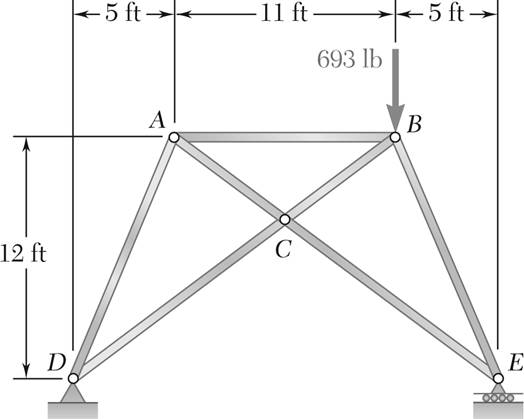
\includegraphics[width=0.5\textwidth,
	           height=0.4\textheight,
		   keepaspectratio]{fig.png}
  \caption*{Temporary Platform}
\end{figure}

\iftoggle{flagSoln}{%
\vspace{.5cm}
\rule{\textwidth}{.4pt}
\vspace{.5cm}
\textbf{Solution:}
\begin{figure}[ht!]
  \centering
  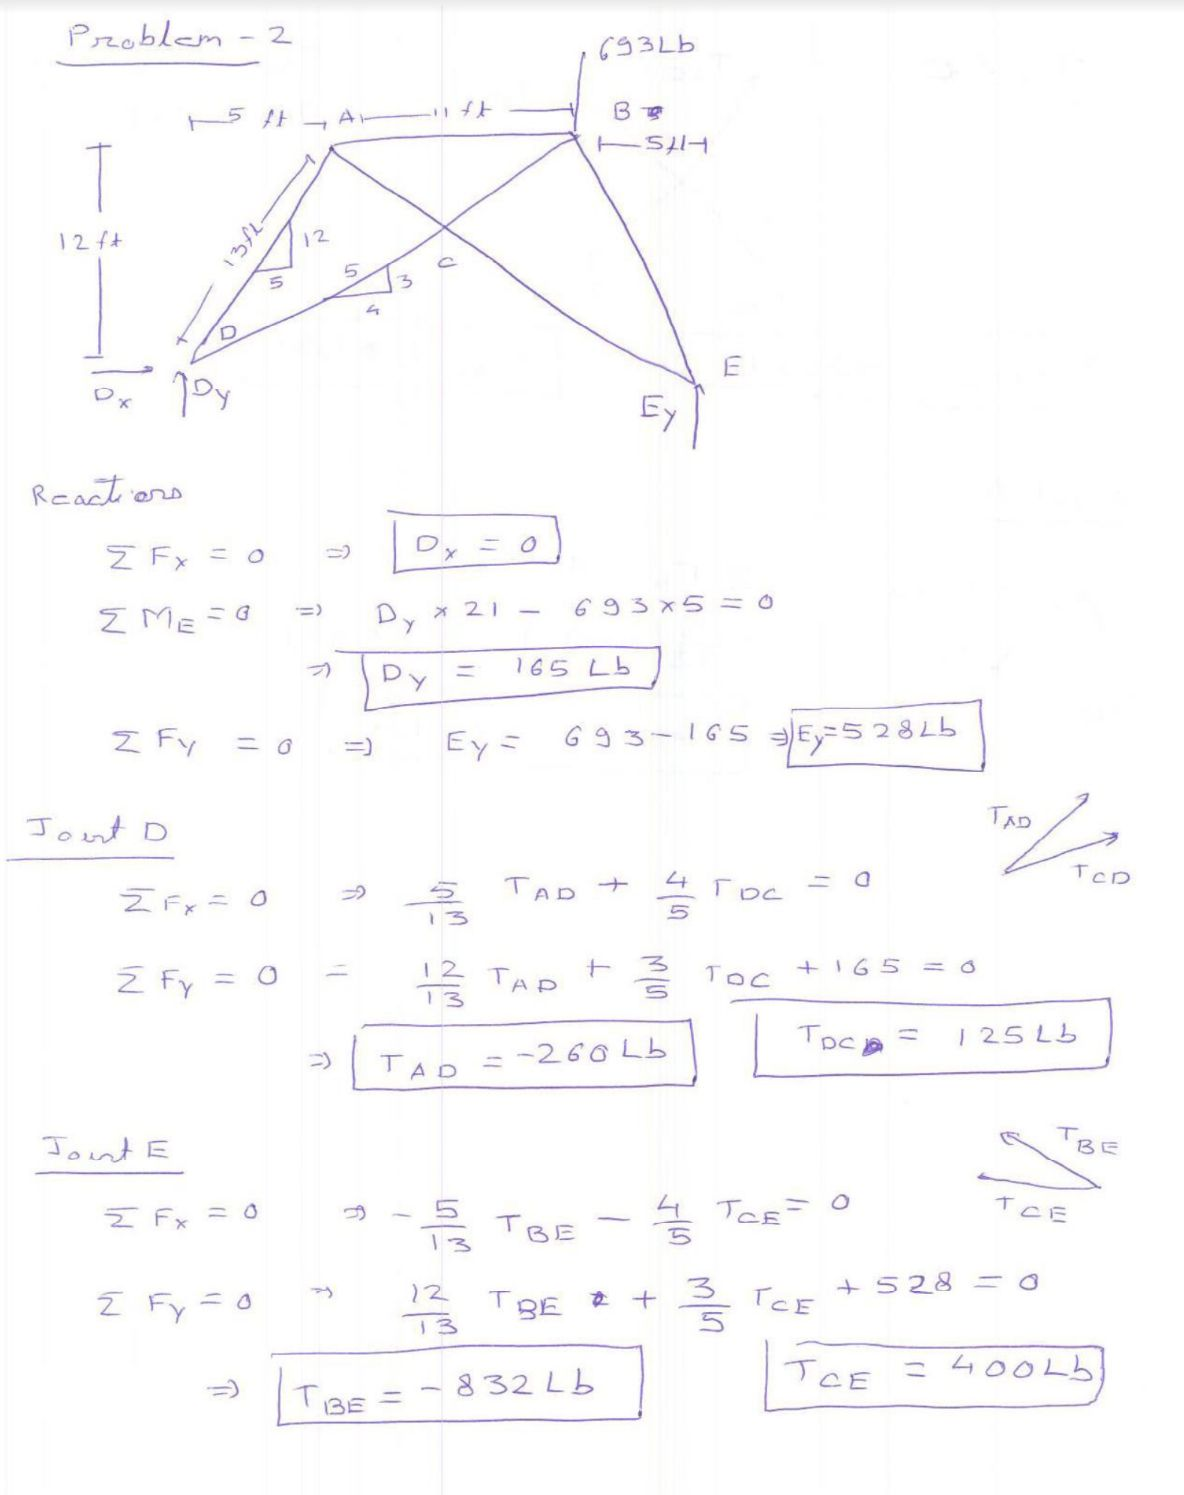
\includegraphics[width=0.4\textwidth,
	           height=0.4\textheight,
		   keepaspectratio]{solna.png}
  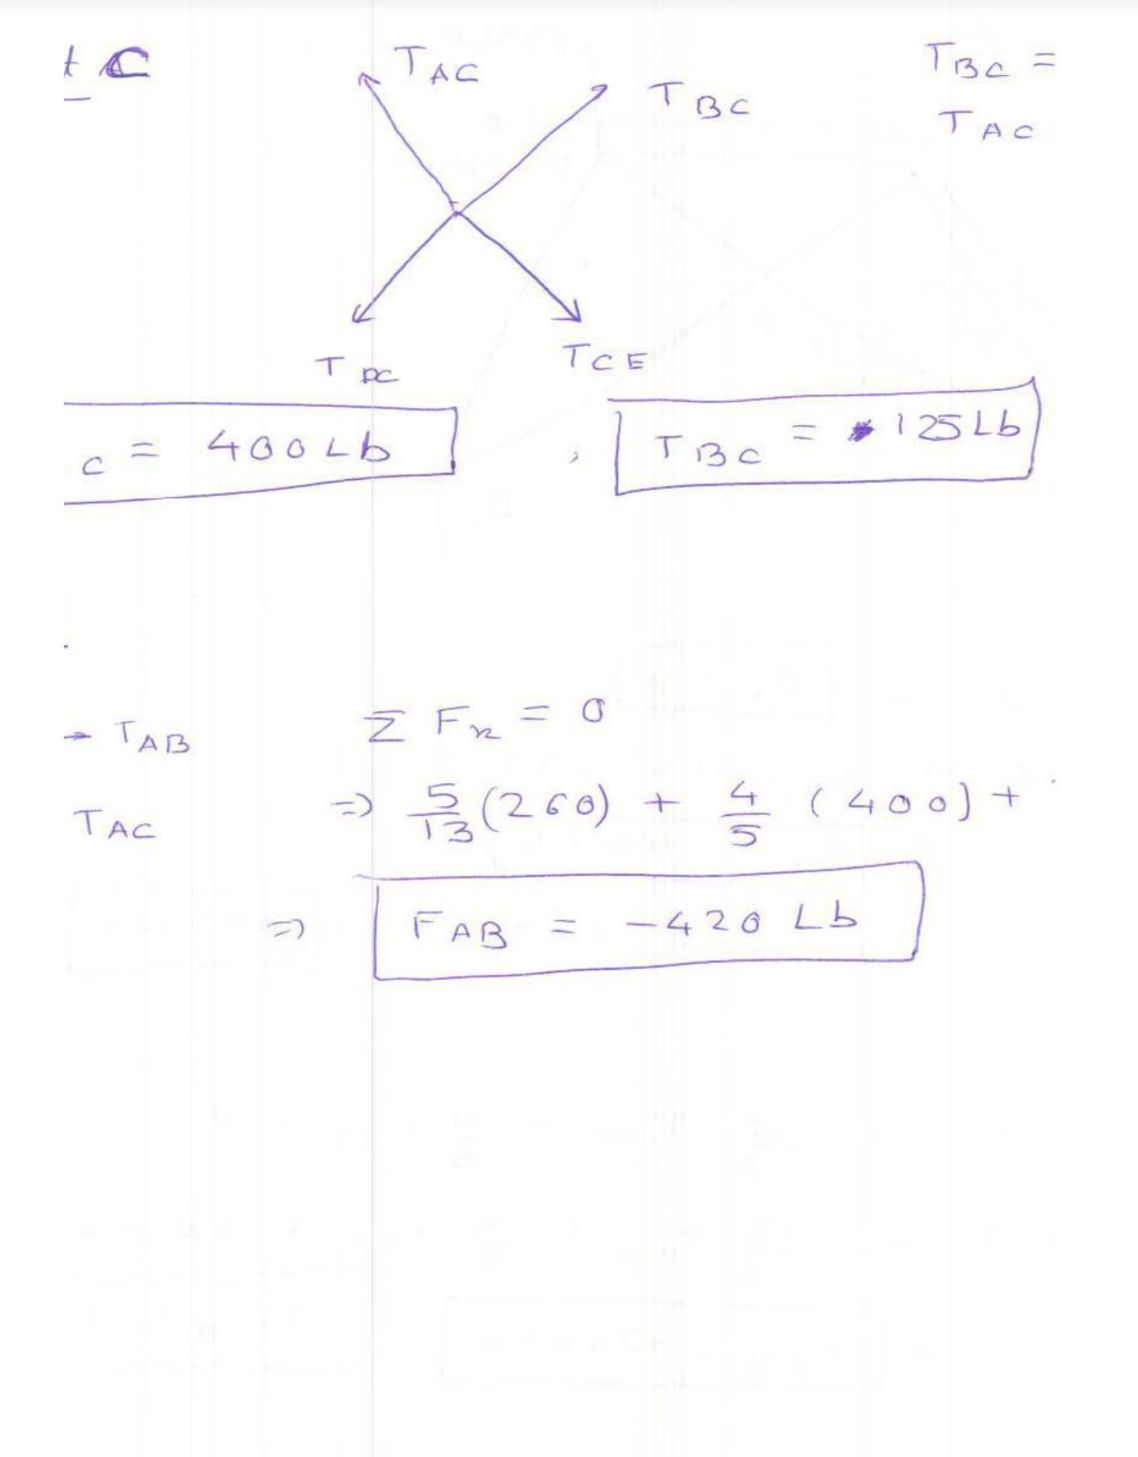
\includegraphics[width=0.4\textwidth,
	           height=0.4\textheight,
		   keepaspectratio]{solnb.png}
\end{figure}
}{%
}%
